%%%%%%%%%%%%%%%%%%%%%%%%%%%%%%%%%%%%%%%%%%%%%%%%%%%%%%%%%%%%%%%%%%%%%%%%%%%%%
%% Descr:       Vorlage für Berichte der DHBW-Karlsruhe, Ein Kapitel
%% Author:      Prof. Dr. Jürgen Vollmer, vollmer@dhbw-karlsruhe.de
%% $Id: kapitel2.tex,v 1.5 2017/10/06 14:02:51 vollmer Exp $
%%  -*- coding: utf-8 -*-
%%%%%%%%%%%%%%%%%%%%%%%%%%%%%%%%%%%%%%%%%%%%%%%%%%%%%%%%%%%%%%%%%%%%%%%%%%%%%%%

\chapter{Technologien}
In diesem Kapitel werden alle für das Verständnis notwendigen und verwendeten Technologien aufgeführt und genauestens erläutert.
\\Die durch die Programmiersprache \textit{C\#}, von Microsoft, zur Verfügung gestellte Technologie \textit{WPF} wird in folgendem Auskunft über 
allgemeine Informationen, Funktionsweise, Einsatzgebiete und deren untergeordneten Technologien konkretisiert. 
\\Mit den vorab getätigten Überlegungen zu Zeichentechnologien die kompatibel mit \textit{C\#}, bzw. \textit{WPF} waren kam man zu der von Microsoft
entwickelten Zeichentool System.Drawing, die ebenso präzisiert wird.
%WPF: https://de.wikipedia.org/wiki/Windows_Presentation_Foundation am 08.04.2020, um 23:55 Uhr
%WPF: [WPF]https://docs.microsoft.com/de-de/dotnet/framework/wpf/getting-started/introduction-to-wpf-in-vs am 08.04.2020, um 23:55 Uhr
%WPF: https://www.wpf-tutorial.com/de/1/uber-wpf/was-ist-wpf/ am 08.04.2020, um 23:55 Uhr
%WPF: https://docs.microsoft.com/de-de/dotnet/framework/wpf/introduction-to-wpf am 08.04.2020, um 00:20 Uhr
\section{WPF (Mikka Jenne)}
\ac{WPF} in Visual Studio bietet Entwicklern ein einheitliches Programmiermodell zum 
Erstellen von Line-of-Business-Desktopanwendungen unter Windows. \cite{wpfmicrosoft.2020a} 
\\Das Grafik-Framework \acs{WPF}, sowie die Entwicklungsumgebung Visual Studio sind beides Produktionen des Unternehmens Microsoft.
Von Microsoft wird es als das Framework zur Erstellung von Desktop-Clientanwendungen für Windows mit visuell herausragenden 
Benutzerflächen umworben.
\linebreak
Der Kern von \textit{WPF} ist eine auflösungsunabhängige und vektorbasierte Rendering-Engine, die die Leistungsfähigkeit 
moderner Grafikhardware nutzt. [WPF Kern] Dieser Kern wird durch \textit{WPF} um mehrere Features zur Entwicklung von Anwendungen 
erweitert. Zu den Erweiterungen des \textit{WPF}-Kerns zählen unteranderem die Beschreibungssprache Extensible Application Markup Language \textit{XAML}, 
die in der nächsten Sektion konkretisiert wird, diverse Steuerelemente, Datenbindungen, 2D- und 3D-Grafik, Animationen, Vorlagen, Dokumente, Texte 
und Typographie.
\\Die Anlehnung von \textit{WPF} an \textit{.NET}-Typen ist sehr stark, da \textit{WPF} eine Teilmenge von \textit{.NET} ist. Die Typen von \textit{.NET} sind zum größten Teil im 
Namespace System.Windows, welcher im Nachgang noch genauer aufgezeigt wird, wiederzufinden. 
\\Das Grafik-Framework kann in zweierlei Programmiersprachen implementiert werden, zum einen unter der Nutzung von \textit{C\#} und zum anderen kann 
Visual Basic verwendet werden. 
\\Microsoft entwickelte viele Technologien und Frameworks, die die themenübergreifende Nutzung möglich machen, bzw. die Einfachheit besitzen 
durch die vorhandenen Grundlagen viele dieser Technologien nutzen zu können ohne neues Wissen aneignen zu müssen, da die Grundlagen identisch 
sind. Zu diesen Technologien gehören \textit{ASP.NET} und Windows Forms als Vorgänger von \textit{WPF}.
%Allgemein was das ist
%Wie es funktioniert, was es macht
%Welche Möglichkeiten es mit WPF gibt
%Welche verfügbaren Komponenten es dazu gibt (XAML, etc.) 
\subsection{XAML - Extensible Application Markup Language} % https://de.wikipedia.org/wiki/Extensible_Application_Markup_Language am 01.04.2020, um 18:00 Uhr
Allgemein ist \ac{XAML} eine Beschreibungssprache zur Gestaltung grafischer Benutzeroberflächen, entwickelt von Microsoft. Die neue deklarative 
Sprache wurde für das Framework \textit{.Net 3.0} in Windows Presentation Foundation \textit{WPF} für \textit{WPF}-Windows-Anwendungen entwickelt. \cite{wpf.2020a} 
\\Die Extensible Application Markup Language ist eine XML-basierende Sprache, die verwendet wird, um Benutzeroberflächen, Verhaltensweisen, 
Animationen, grafische Elemente etc. zu definieren. 
\subsection*{Window - Fenster}
Ein Code-Template eines standardmäßigen Fensters \textit{Window} sieht wie folgt aus und wird so als Basis-XAML zur Verfügung gestellt.
% \begin{figure}[hbt!]
    % \centering
    % 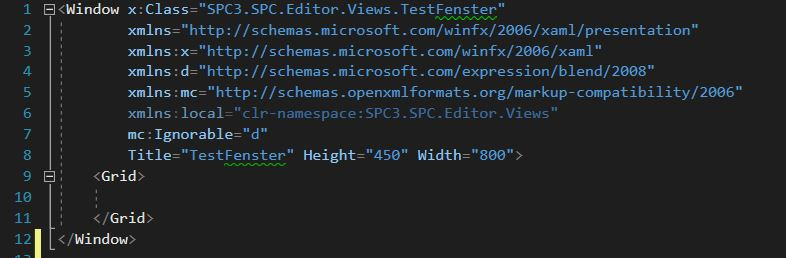
\includegraphics[width=15cm,height=10cm,keepaspectratio]{3Technologien/Bilder/XAML-CodeSnippet}
    % \caption{Window-Template}
% \end{figure}
\begin{lstlisting}[language=XML,
    frame=single,           % Ein Rahmen um den Code
    framexleftmargin=15pt,  % Rahmen link von den Zahlen
    style=algoBericht,
    label={window-template},
    captionpos=b,           % Caption unter den Code setzen
caption={Window-Template}]
<Window x:Class="WpfApplication1.Window1"
    xmlns="http://schemas.microsoft.com/winfx/2006/xaml/presentation"
    xmlns:x="http://schemas.microsoft.com/winfx/2006/xaml"
    Title="Window1" Height="300" Width="300">
    <Grid>

    </Grid>
</Window>
\end{lstlisting}
Der oben aufgeführte Ausschnitt zeigt eine \textit{XAML}-Datei, die ein vorgefertigtes Template von Microsoft darstellt. 
Bei Erstellung einer neuen Datei, bzw. einer Benutzeroberfläche, wird dieses Template zur Verfügung gestellt. Es
beinhaltet zu Anfang alle relevanten Informationen über Größe des Fensters und dessen Design. Ein Grid, 
welches ebenso in dem Template vorhanden ist, erfüllt die Funktion eines Koordinators. Das bedeutet, dass auf der 
Oberfläche ein Raster angelegt wird, welches die Positionen verschiedener Komponenten und Elementen koordiniert. So kann 
allen Elementen ein fester Platz, an dem es angeordnet sein soll, zugewiesen werden.
\linebreak
Ebenso umfasst ein \textit{Window} einen hypothetischen Container, bzw. ein Grundgerüst, welches als Repräsentation 
verschiedener Seiten \textit{Page} verwendet wird. Die Basisklasse stellt einen Standardrahmen, sowie eine Titelzeile, einem 
Maximierungs-, Minimierungs- und Schließknopf zur Verfügung.
\subsection*{Page - Seite}
Neben dem Template für ein Fenster gibt es anderweitige Templates, um das Erscheinungsbild von Oberflächen zu gestalten.
Zum Beispiel gibt es, wie im Absatz darüber erwähnt, die sogenannten Pages, die im Template sichtlich das Markup \textit{Window} 
durch \textit{Page} ersetzen. Der Funktionsunterschied is jedoch enorm, wogegen das Window ein Grundgerüst mitliefert, zeigt die 
Seite nur die Oberfläche ohne Rahmen, die verwendet werden kann.
% \begin{figure}[hbt!]
    % \centering
    % 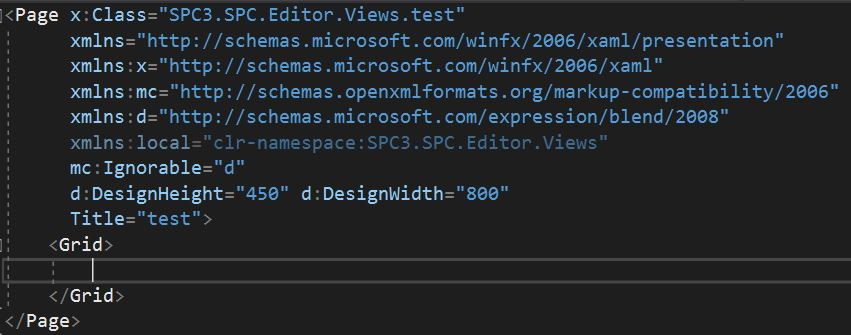
\includegraphics[width=15cm,height=10cm,keepaspectratio]{3Technologien/Bilder/PageXAML}
    % \caption{Page-Template}
% \end{figure}
\pagebreak
\begin{lstlisting}[language=XML,
    frame=single,           % Ein Rahmen um den Code
    framexleftmargin=15pt,  % Rahmen link von den Zahlen
    style=algoBericht,
    label={page-template},
    captionpos=b,           % Caption unter den Code setzen
caption={Page-Template}]
<Page x:Class="WpfApplication1.Page1"
    xmlns="http://schemas.microsoft.com/winfx/2006/xaml/presentation"
    xmlns:x="http://schemas.microsoft.com/winfx/2006/xaml"
    Title="Page1" Height="300" Width="300">
    <Grid>

    </Grid>
</Page>
\end{lstlisting}
\subsection*{UserControl - Benutzersteuerelement}
Eine dritte From der Repräsentation ist das sogenannte \textit{UserControl} (dt. Benutzerkontrolle), welches im Prinzip eine 
Mischung aus einem Window und einer Seite ist. Der Unterschied zwischen den einzelnen Elementen ist lediglich das Markup,
bzw. die Namensgebung \textit{UserControl}. 
\begin{lstlisting}[language=XML,
    frame=single,           % Ein Rahmen um den Code
    framexleftmargin=15pt,  % Rahmen link von den Zahlen
    style=algoBericht,
    label={usercontrol-template},
    captionpos=b,           % Caption unter den Code setzen
caption={UserControl-Template}]
<UserControl x:Class="WpfApplication1.UserControl1"
    xmlns="http://schemas.microsoft.com/winfx/2006/xaml/presentation"
    xmlns:x="http://schemas.microsoft.com/winfx/2006/xaml"
    Title="UserControl1" Height="300" Width="300">
    <Grid>

    </Grid>
</UserControl>
\end{lstlisting}
% https://www.c-sharpcorner.com/UploadFile/1e050f/grid-layout-in-wpf/ 
\subsection*{Grid}
Ein Grid ist ein Rasterelement in \textit{WPF} und teilt eine Seite oder ein Fenster in eine vorab definierte Anzahl von Zeilen und Spalten.
Das Raster ist ein sehr leistungsfähiges und nützliches Layout in WPF. 
Damit können untergeordnete Elemente in Zellen angeordnet werden, die durch Zeilen und Spalten definiert sind. 
Wenn ein neues XAML-Dokument erstellt wird, fügt Visual Studio automatisch ein Raster als ersten Container innerhalb des 
Fensterelements hinzu. Dieses vorgegebene Template kann durch \textit{Grid.ColumnDefinitions} in Spalten und durch \textit{Grid.RowDefinitions} 
in Zeilen unterteilt werden, wie dem folgenden Code-Ausschnitt zu entnehmen ist. \cite{wpftutorial.2020a}
\begin{lstlisting}[language=XML,
    frame=single,           % Ein Rahmen um den Code
    framexleftmargin=15pt,  % Rahmen link von den Zahlen
    style=algoBericht,
    label={gridtemplate},
    captionpos=b,           % Caption unter den Code setzen
caption={Grid-Template}]
<Grid.ColumnDefinitions>
	<ColumnDefinition/>
	<ColumnDefinition/>
</Grid.ColumnDefinitions>
<Grid.RowDefinitions>
	<RowDefinition />
	<RowDefinition />
</Grid.RowDefinitions>
\end{lstlisting}
% \begin{figure}[hbt!]
    % \centering
    % 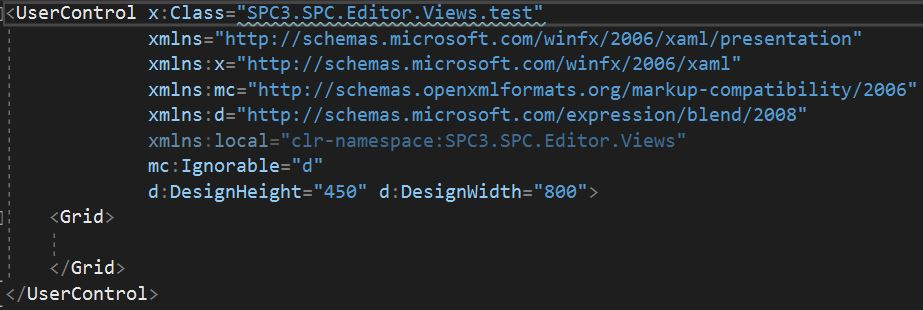
\includegraphics[width=15cm,height=10cm,keepaspectratio]{3Technologien/Bilder/UCXAML}
    % \caption{UserControl-Template}
% \end{figure}

% https://docs.microsoft.com/de-de/dotnet/api/system.windows?view=netcore-3.1 
\subsection{System.Windows}
\textit{System.Windows} ist ein in WPF deklarierter Namespace. Eine Bibliothek die viele essentiellen Methoden, verschiedene Klassen und 
WPF-Basiselementklassen zur Verfügung stellt. \cite{wpfmicrosoftwindow.2020a}
die das WPF-Eigenschaftensystem 
und die zugehörige Ereignislogik unterstützen, sowie andere Typen bereit, die häufig vom WPF-Kern und -Framework benötigt werden.
Die API, engl. Application Programming Interface, stellt zum Beispiel eine Drag \& Drop - Funktion bereit, die Hilfsmethoden und Felder für die Einleitung 
von Drag \& Drop-Vorgängen bietet. Zusätzlich beinhaltet diese Schnittstelle eine Methode zum Starten eines solchen Vorgangs und verwaltet 
und überwacht das Hinzufügen und Entfernen von Drag \& Drop-bezogenen Ereignishandlern.
\\Darüberhinaus gibt es viele weitere Methoden die über diesen Namespace zur Verfügung gestellt werden. 
\\Ein weiterer Namespace der in der Entwicklung verwendet wurde ist der sogenannte \textit{System.Collections}-Namespace, der in folgendem 
kurz beschrieben und mit einem Beispiel dargelegt wird.
% https://docs.microsoft.com/de-de/dotnet/api/system.collections?view=netcore-3.1
\subsection{System.Collections}
Der \textit{System.Collections}-Namespace enthält Schnittstellen und Klassen, die verschiedene Auflistungen von Objekten definieren, 
z.B. \textit{Listen}, \textit{Warteschlangen}, \textit{Bitarrays}, \textit{Hashtabellen} und Wörterbücher. \cite{wpfmicrosoftcollection.2020a}
Ein bekannter Parameter dieser Schnittstelle ist die \textit{ArrayList}, eine Anreihung von Feldern, die nach Anforderungen, bzw. nach Gebrauch
beliebig erweitert werden kann und Datenstrukturen der gleichen Form speichert.
\\Zur Implementierung der Hauptanwendung, das Zeichnen der Schaltpläne, werden die Schnittstellen des 
\textit{System.Drawings}-Namespaces verwendet.  

% https://docs.microsoft.com/de-de/dotnet/api/system.drawing?view=dotnet-plat-ext-3.1#classes 
\subsection{System.Drawing}
Der \textit{System.Drawing}-Namespace ist für die Darstellung von bestimmten Textformaten, Anzeigen von Graphiken 
durch \textit{Bitmaps} oder \textit{Icons} und ermöglicht den Zugriff auf die grundlegensten Grafikfunktionen. \cite{wpfmicrosoftdrawing.2020a} Durch weitere Namepsaces können diese 
Funktionen erweitert, bzw. verfeinert werden. Es werden über diesen Namespace auch Methoden zur händischen Zeichnung 
von Graphiken angeboten. 

\section{MVVM (Simon Leitl)}
\label{chap:MVVM}

Model-View-ViewModel ist ein Architekturmuster welches Entwicklern als Vorlage dient und hilft grafische Oberflächen standardisiert und strukturiert zu entwickeln. MVVM wird als Weiterentwicklung bekannter Architekturmuster wie MVC betrachtet. MVVM ist 2005 im Zuge der Entwicklung von WPF entstanden und ist mittlerweile bestandteil von Universal Apps und Webframeworks. MVVM trennt die Benutzeroberflächen von der Logik. Dabei wird die Logik in sogenannten ViewModel Klassen dargestellt. Die Benutzeroberfläche bindet sich an die Properties der ViewModel Klassen und erhält fast keinen prozeduralen Code. Setzt man das MVVM Pattern richtig um, enthalten die ViewModel Klassen keine Benutzeroberflächen Elemente. Dies ist ein großer Vorteil für das durchführen von Unit Tests. Die ViewModel Klasse selbst stellt öffentliche Properties und Commands zur Verfügung, an welche sich die View binden kann. Die Ebenen sind in \ref{pic:mvvm-pattern} zu sehen.
\begin{figure}[ht]
    \centering
    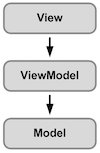
\includegraphics{3Technologien/Bilder/mvvmpattern}
    \caption{MVVM Pattern}
    \label{pic:mvvm-pattern}
\end{figure}
\linebreak
\\Die View Ebene wird zum Darstellen genutzt, die ViewModel Ebene enthält die Logik durch Commands und zuletzt das Model, welches die Daten enthält. 
\\Die Kommunikation zwischen der Benutzeroberfläche und der Logik wird durch sogenannte Bindings durchgeführt. Dabei werden Bestandteile der Benutzeroberfläche an das ViewModel oder bestimmte Commands des ViewModel, also der Logik gebindet. Über das Binding verläuft dann die Kommunikation zwischen den Komponenten. Dabei muss das Binding in der XAML Datei der View, einem Objekt zugewiesen werden, wie in Code-Beispiel ~\ref{xaml-binding} zu sehen ist. Die Zuweisung ist der Name einer Funktion, die im ViewModel vorhanden ist.
\\
\begin{lstlisting}[language=XML,
    frame=single,           % Ein Rahmen um den Code
    framexleftmargin=15pt,  % Rahmen link von den Zahlen
    style=algoBericht,
    label={xaml-binding},
    captionpos=b,           % Caption unter den Code setzen
caption={Binding in XAML}]
    <TextBlock Margin="3" Text="{Binding ViewModelNameList}"/>
\end{lstlisting}
Die Funktion wird dabei dem TextBlock aus dem Code-Beispiel ~\ref{xaml-binding} als Quelle zugewiesen. Über diese Funktion werden nun die Daten, die innerhalb des Textblocks auf der Oberfläche angezeigt werden, bezogen. Um die Daten im ViewModel entsprechend zur Verfügung zu stellen, wird eine Funktion benötigt. Diese Funktion besitzt einen Getter Methode, um die Daten über einen return auszugeben. Im Code-Beispiel \ref{viewmodel-binding} wird diese Funktion dargestellt. Sie enthält eine Liste in der die Namen aller VieModels gespeichert ist. 
\\
\begin{lstlisting}[language=C,
    frame=single,           % Ein Rahmen um den Code
    framexleftmargin=15pt,  % Rahmen link von den Zahlen
    style=algoBericht,
    label={viewmodel-binding},
    captionpos=b,           % Caption unter den Code setzen
    caption={Binding im ViewModel}]
public ObservableCollection<String> ViewModelNameList
{
    get { return _viewModelNameList; }
}
\end{lstlisting}
Die Funktion gibt die Namen eines ViewModel als String zurück. Dieser String wird dann innerhalb der TextBox in \ref{xaml-binding} abgebildet.
\\ Alle ViewModel die Funktionen für Bindings enthalten erben von der ViewModelBase Klasse. Dadurch wird die, in der ViewModelBase enthaltene \textit{INotifyPropertyChanged} Funktion implementiert. Diese ist Notwendig um Anzeigen auf der Oberfläche während der Laufzeit der Anwendung zu ändern und zu aktualisieren. 
Durch die \textit{INotifyPropertyChanged} erkennt die Anwendung zur Laufzeit Änderungen an der Oberfläche oder der Logik. Findet eine Änderung statt so ist die Funktion dafür verantwortlich, alle Teilnehmer des Bindings zu informieren und die Änderungen zu aktualisieren. \cite{mvvm.2010s}

\subsection{MVVM Light Framework}
MVVM Light ist ein Framework, das dazu entwickelt wurde MVVM Architekturen in Windows Universal, WPF, Silverlight, Xamarin.iOS, Xamarin.Android und Xamarin.Forms zu entwickeln. Dabei hilft das Framework bei der Erstellung der Strukturen innerhalb eines Projekts. Somit haben die Entwickler eine Basis, auf die sie sich bei der Umsetzung beziehen können. Dadurch erhält die Anwendung eine einfache und saubere Wartbarkeit sowie eine einfache Erweiterbarkeit. MVVM Light hilft dabei, die View vom Model zu trennen. Ein weiterer Vorteil des Frameworks sind die verbesserten Testmöglichkeiketen für das entwickelte Projekt. Es erstellt testbare Anwendungen welche über eine dünnere Benutzeroberfläche verfügen. \cite{mvvmLight.2020a}

\endinput
%%%%%%%%%%%%%%%%%%%%%%%%%%%%%%%%%%%%%%%%%%%%%%%%%%%%%%%%%%%%%%%%%%%%%%%%%%%%%%%
